%----------------------------------------------------------------------------------------
%	PACKAGES AND THEMES
%----------------------------------------------------------------------------------------

\documentclass[aspectratio=169]{beamer}
\mode<presentation> {
	\usetheme{Boadilla}
}
\definecolor{lmugreen}{RGB}{0, 136, 58}
\usecolortheme[named=lmugreen]{structure}
\usepackage{graphicx}
\usepackage{booktabs}
\usepackage[english]{babel}
\usepackage[utf8]{inputenc}
\usepackage{amsmath,amssymb}
\usepackage{float}
\usepackage{hyperref}
\newcommand{\gray}{\rowcolor[gray]{.90}}
\usepackage{verbatim}
\usepackage{textpos}
\usepackage[default]{sourcesanspro}
\usepackage{cases}

% Caption
\usepackage{caption}
\DeclareCaptionFont{tiny}{\tiny}
\captionsetup{font=scriptsize,labelfont=scriptsize,justification=centering}

% Automatic section outline slide
\AtBeginSection[]{
	\begin{frame}[noframenumbering, plain]
	\frametitle{Outline}
	\setcounter{tocdepth}{1}
	\tableofcontents[currentsection]
\end{frame}
}

% Remove navigation symbols
\beamertemplatenavigationsymbolsempty

% R listings
\usepackage{listings}
\lstset{
language=R,
basicstyle=\scriptsize\ttfamily,
commentstyle=\ttfamily\color{gray},
backgroundcolor=\color{white},
showspaces=false,
showstringspaces=false,
showtabs=false,
tabsize=2,
captionpos=b,
breaklines=false,
breakatwhitespace=false,
title=\lstname,
escapeinside={},
keywordstyle={},
morekeywords={},
belowskip = -1.2 \baselineskip,
}

%----------------------------------------------------------------------------------------
%	TITLE PAGE
%----------------------------------------------------------------------------------------

\addtobeamertemplate{frametitle}{}{%
	\begin{textblock*}{100mm}(0.88\textwidth,-0.5cm)
		
\includegraphics[height=1cm,width=2cm]{lmu_logo}
\end{textblock*}}

\title[Trajectron++ Analysis]{Understanding Trajectron++: \\
A Interpretable Performance Analysis Pipeline}

\author[Drauz \& Matrullo]{Simon Drauz and Zoe Matrullo}
\institute[LMU]{LMU Munich}

%----------------------------------------------------------------------------------------
%	DOCUMENT
%----------------------------------------------------------------------------------------

\begin{document}

%--- Slide 1: Title -------------------------------------------------------------
{
\usebackgroundtemplate{
\includegraphics[width=\paperwidth]{lmu-background.pdf}}
\begin{frame}
\begin{columns}
	\begin{column}{0.4\textwidth}
		\vspace*{3cm}
		\textbf{\textcolor{white}{\Large 
		\\ Understanding Trajectron++:\\
A Per-Trajectory Performance Analysis \\}}
		\vspace{1cm}
		\textcolor{white}{\footnotesize Simon Drauz and Zoe Matrullo \\
			\today}
	\end{column}
	\begin{column}{0.49\textwidth}
		\vspace*{2cm}
		\begin{center}
			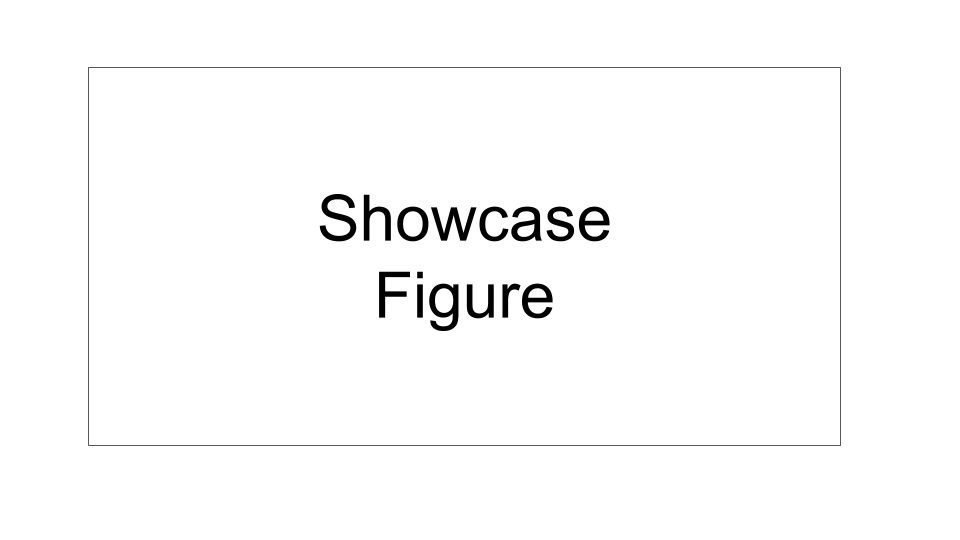
\includegraphics[width=1\textwidth]{showcase_figure.png}
		\end{center}
	\end{column}
\end{columns}
\end{frame}
}

%--- Slide 2: Outline -----------------------------------------------------------
%--- Slide 2: Outline -----------------------------------------------------------

\begin{frame}{Outline}
  \tableofcontents
\end{frame}


%--- Part 1: Motivation ---------------------------------------------------------
%--- Part 1: Motivation (4 min) -------------------------------------------------

\section{Motivation}

%--- Slide: Trajectory Prediction for Autonomous Driving -----------------------
\begin{frame}{Trajectory Prediction for Autonomous Driving}
  \begin{columns}
    \begin{column}{0.55\textwidth}
      \begin{itemize}[<+->]
        \item \textbf{Task:} forecast future $(x, y)$ positions of agents
              (pedestrians, cyclists, motorcyclists, vehicles) from observed past movements
        \item Challenging due to \textbf{complex agent interactions} and influence of \textbf{static context}
        \item Essential for \textcolor{lmugreen}{\textbf{safe path planning}} and \textcolor{lmugreen}{\textbf{collision avoidance}}
              in autonomous vehicles
      \end{itemize}
    \end{column}
    \begin{column}{0.42\textwidth}
      \begin{center}
        
\includegraphics[width=\textwidth]{trajectory_prediction}\\
        \vspace{0.2em}
        {\tiny Source: Salzmann et al.\ (2020)}
      \end{center}
    \end{column}
  \end{columns}
\end{frame}

%--- Slide: Trajectron++ -------------------------------------------------------
\begin{frame}{Trajectron++}
  \begin{columns}
    \begin{column}{0.52\textwidth}
      \begin{itemize}
        \item<1-> State-of-the-art probabilistic trajectory prediction model
              \textnormal{\small[Salzmann et al., 2020]}
        \item<2-> \emph{Spatio-temporal graph encoder}
        \begin{itemize}
          \item LSTM per agent
          \item edges encode agent--agent interactions
        \end{itemize}
        \item<3-> \emph{CVAE decoder}
        \begin{itemize}
          \item Outputs a distribution over future
              trajectories
        \end{itemize}
        \item<4-> Handles \emph{heterogeneous} agent types jointly
              (pedestrian, bicycle, motorcycle, car) and integrates HD map context
        \item<6-> \small \textbf{ADE:} avg.\ L2 distance over all predicted timesteps
        \item<7-> \small \textbf{FDE:} L2 distance at the final predicted timestep
      \end{itemize}
    \end{column}
    \begin{column}{0.45\textwidth}
      \begin{center}
        
\includegraphics[width=\textwidth]{trajectronpp}\\
        {\tiny Source: Salzmann et al.\ (2020)}
      \end{center}
      \onslide<5->{
        \vspace{0.3em}
        \footnotesize
        \textbf{Performance metrics:}\\[0.2em]
        \begin{tabular}{ll}
          \texttt{ml\_ade}     & most-likely ADE \only<8->{\textcolor{lmugreen}{\textbf{$\leftarrow$ used}}}\\
          \texttt{ml\_fde}     & most-likely FDE \\
          \texttt{min\_ade\_5} & best-of-5 ADE \\
          \texttt{nll\_mean}   & neg.\ log-likelihood \\
        \end{tabular}
      }
    \end{column}
  \end{columns}
\end{frame}

%--- Slide: nuScenes -----------------------------------------------------------
\begin{frame}{nuScenes Dataset}
  \begin{columns}
    \begin{column}{0.50\textwidth}
      \begin{itemize}
        \item<1-> 1\,000 urban driving scenes, Boston \& Singapore
        \item<2-> Agent types: pedestrians, cyclists, motorcyclists, vehicles
        \item<3-> Rich sensor suite: camera, LiDAR, radar, GPS, HD map
        \item<4-> Standard split: 700 / 150 / 150 (train / val / test)
        \item<5-> \textbf{Scope:} we predict \emph{pedestrian} trajectories
              only, all agent types serve as scene context
      \end{itemize}
    \end{column}
    \begin{column}{0.47\textwidth}
      \centering
      
\includegraphics[width=0.55\textwidth]{nuscenes_example3}\\[0.15em]
      
\includegraphics[width=0.75\textwidth]{nuscenes_maps}\\[0.1em]
      {\tiny Source: Caesar et al.\ (2020)}

      \onslide<6->{%
        \vspace{0.3em}
        \footnotesize
        \textbf{trajdata} \textnormal{\small[NVLabs]}\\[0.2em]
        \begin{itemize}
          \item Unified interface to many trajectory datasets
                (nuScenes, ETH/UCY, \ldots)
          \item[$\Rightarrow$] Our analysis pipeline applies to
                \emph{any} trajdata-supported dataset
        \end{itemize}
      }
    \end{column}
  \end{columns}
\end{frame}

%--- Slide: Research Questions -------------------------------------------------
\begin{frame}{Challenges and Research Questions}
  \begin{columns}
    \begin{column}{0.52\textwidth}
      \begin{itemize}[<+->]
        \item Some trajectories are inherently hard, others trivially
              easy---but \emph{why?}
        \item A single average ADE/FDE gives no insight into reasons
              for failure and success
        \item No understanding of which trajectory or scene characteristics
              drive per-trajectory prediction error
      \end{itemize}
      \vspace{0.4em}
      \onslide<4->{$\Rightarrow$ \textbf{\textcolor{lmugreen}{Three research questions:}}}
    \end{column}
    \begin{column}{0.45\textwidth}
      \begin{enumerate}
        \item<5-> Which trajectory and scene characteristics affect model
              performance?
        \item<6-> What are the \emph{success and failure modes} that explain
              model performance?
        \item<7-> How do model settings (history window, prediction horizon,
              attention radius) affect performance?
      \end{enumerate}
    \end{column}
  \end{columns}
\end{frame}


%--- Part 2: Analysis Pipeline --------------------------------------------------
%--- Part 2: Analysis Pipeline (4 min) -----------------------------------------

\section{Analysis Pipeline}

%--- Slide 5 -------------------------------------------------------------------
\begin{frame}{Two Analysis Paths}
  % TODO: pipeline diagram (TikZ or figure)
  \begin{columns}
    \begin{column}{0.48\textwidth}
      \textbf{Track 1 — Full Dataset}\\[0.4em]
      Train Trajectron++ $\to$ per-trajectory ADE\\
      $\to$ join trajectory + scene characteristics\\
      $\to$ interpretable models $\to$ feature effects\\
      $\to$ performance regime clustering\\
      $\to$ cluster inspection
    \end{column}
    \begin{column}{0.48\textwidth}
      \textbf{Track 2 — Mini Dataset (Settings Sweep)}\\[0.4em]
      Cartesian sweep over model settings\\
      $\to$ combine runs\\
      $\to$ interpretable models\\
      $\to$ feature effects with settings as predictors\\
      \hspace{1em}(trajectory/scene chars as controls)
    \end{column}
  \end{columns}
  \vspace{0.5em}
  \footnotesize Clustering + cluster inspection run only on the full-dataset path.
\end{frame}

%--- Slide 6 -------------------------------------------------------------------
\begin{frame}{Trajectron++ Modification}
  \begin{columns}
    \begin{column}{0.46\textwidth}
      \textbf{Standard Trajectron++}
      \begin{itemize}[<+->]
        \item Evaluation outputs \emph{batch-averaged} ADE / FDE
        \item No way to link prediction error back to an
              individual trajectory
        \item Cannot study what makes a trajectory hard or easy
      \end{itemize}
    \end{column}
    \begin{column}{0.50\textwidth}
      \onslide<4->{\textbf{Our Modification}}
      \begin{itemize}
        \item<5-> Recover \emph{individual trajectory loss \& characteristics}\\
              by modifying Trajectron++'s evaluation loop
        \item<6-> \texttt{data\_idx}: stable trajdata identifier,
              used to join evaluation output with computed
              trajectory \& scene characteristics
      \end{itemize}
    \end{column}
  \end{columns}
\end{frame}


%--- Part 3: Data Preparation ---------------------------------------------------
%--- Part 3: Data Preparation (6 min) ------------------------------------------

\section{Data Preparation}

%--- Slide 7 -------------------------------------------------------------------
\begin{frame}{Dataset Overview}
  % TODO: nuScenes dataset stats, split sizes, agent counts, scene counts
  \begin{itemize}
    \item \ldots
  \end{itemize}
\end{frame}

%--- Slide 8 -------------------------------------------------------------------
\begin{frame}{Target Distribution \& Transformation}
  % TODO: histogram of ml_ade; motivation for log transform / Gamma link
  \begin{itemize}
    \item \ldots
  \end{itemize}
\end{frame}

%--- Slide 9 -------------------------------------------------------------------
\begin{frame}{Feature Selection via Mutual Information}
  % TODO: MI bar chart; selected vs. dropped features
  \begin{itemize}
    \item \ldots
  \end{itemize}
\end{frame}

%--- Slide 10 ------------------------------------------------------------------
\begin{frame}{Handling Multicollinearity with VIF}
  % TODO: VIF table before/after; which features were removed/combined
  \begin{itemize}
    \item \ldots
  \end{itemize}
\end{frame}


%--- Part 4: Interpretable Modeling ---------------------------------------------
%--- Part 4: Interpretable Modeling (8 min) ------------------------------------

\section{Interpretable Modeling}

\begin{frame}{Analysis Pipeline}
  \vfill\pipelinehighlight{2}\vfill
\end{frame}

%--- Slide: Why interpretable models? ------------------------------------------
\begin{frame}{Why Interpretable Models?}
  \begin{itemize}[<+->]
    \item We have per-trajectory \texttt{ml\_ade} — but raw error values
          alone do not tell us \emph{why} some trajectories are hard
    \item A black-box model can predict ADE well but gives no insight
          into which features drive it or in which direction
    \item \textbf{Interpretable models} let us directly read off feature
          effects: how does speed, heading change, or scene density
          affect prediction error?
    \item This turns ADE into actionable understanding of model
          behaviour
  \end{itemize}
\end{frame}

%--- Slide: GAM and XGBoost ---------------------------------------------------
\begin{frame}{GAM and XGBoost}
  We tested two interpretable modeling approaches --- either can be used
  for the analysis.
  \vspace{0.5em}
  \begin{columns}[t]
    \begin{column}{0.48\textwidth}
      \textbf{GAM (Generalized Additive Model)}
      \visible<2->{\begin{itemize}[<+->]
        \item Models target as a sum of smooth functions: $f(x) = \sum_j s_j(x_j)$
        \item One spline per feature — no interaction terms
        \item p-values for significance testing
        \item Directly readable smooth effects
      \end{itemize}}
    \end{column}
    \begin{column}{0.48\textwidth}
      \textbf{XGBoost}
      \visible<3->{\begin{itemize}[<+->]
        \item Gradient-boosted decision trees
        \item Flexibly captures non-linearities
              and feature interactions
        \item Post-hoc interpretation via SHAP values
      \end{itemize}}
    \end{column}
  \end{columns}
\end{frame}

%--- Slide: Additive effects & SHAP -------------------------------------------
\begin{frame}{Interpreting the Models: Additive Effects \& SHAP Values}
  \begin{columns}[t]
    \begin{column}{0.48\textwidth}
      \textbf{GAM — Additive Effects}
      \begin{itemize}[<+->]
        \item The model is a sum of smooth terms:
              $\hat{y} = \sum_j \hat{s}_j(x_j)$
        \item Each $\hat{s}_j$ directly shows how feature $j$
              affects \texttt{ml\_ade} — no post-hoc step needed
        \item Confidence bands from the spline fit
      \end{itemize}
    \end{column}
    \begin{column}{0.48\textwidth}
      \textbf{XGBoost — SHAP Values}
      \begin{itemize}[<+->]
        \item Each prediction is decomposed into per-feature
              contributions post-hoc
        \item \emph{Local:} why was this trajectory's ADE high?
        \item \emph{Global:} mean $|$SHAP$|$ gives feature
              importance and direction
      \end{itemize}
    \end{column}
  \end{columns}
  \vspace{0.5em}
\end{frame}

%--- Slide 12 ------------------------------------------------------------------
\begin{frame}{Validating the Tuning Procedure — Nested Resampling}
  \begin{itemize}
    \item \textbf{Problem:} hyperparameter tuning risks overfitting to a
          particular data split
    \item \textbf{Solution:} nested cross-validation
    \begin{itemize}
      \item Outer folds: evaluate generalization of the full tuning procedure
      \item Inner folds: tune hyperparameters on each outer-fold training set via cross-validation
    \end{itemize}
    \item OOF evaluation: inspect out-of-fold predictions for instability,
          outlier folds, bias
    \item \textbf{Conclusion:} tuning generalises stably $\to$ proceed to
          full-data tuning + refit
  \end{itemize}
  \vspace{0.4em}
  \footnotesize Final models are refit on \emph{all} data with optimal
  hyperparameters — no held-out test set, because the goal is understanding,
  not unbiased prediction.
\end{frame}

%--- Slide: GAM Variant Selection ----------------------------------------------
\begin{frame}{GAM Variant Selection}
  \begin{columns}[t]
    \begin{column}{0.44\textwidth}
      \textbf{Three candidates:}
      \begin{itemize}[<+->]
        \item \textbf{LinearGAM} — fitted on raw \texttt{ml\_ade}
        \item \textbf{LinearGAM (log)} — fitted on
              $\log(\texttt{ml\_ade})$, evaluated on original scale
        \item \textbf{GammaGAM} — Gamma distribution with log link,
              suited for positive right-skewed targets
      \end{itemize}
      \vspace{0.5em}
      \onslide<2->{Selection criterion: lowest mean outer-fold RMSE
      (original scale).}
    \end{column}
    \begin{column}{0.53\textwidth}
      \onslide<2->{
      \renewcommand{\arraystretch}{1.3}
      \begin{tabular}{lccc}
        \toprule
        \textbf{Variant} & \textbf{RMSE} & \textbf{R$^2$} & \textbf{MAE} \\
        \midrule
        \textcolor{lmugreen}{\textbf{LinearGAM}} & \textcolor{lmugreen}{\textbf{0.440}} & \textcolor{lmugreen}{\textbf{0.515}} & \textcolor{lmugreen}{0.268} \\
        LinearGAM (log)  & 0.444          & 0.506          & \textbf{0.255} \\
        GammaGAM         & 0.475          & 0.434          & 0.277 \\
        \bottomrule
      \end{tabular}\\[0.4em]
      \footnotesize Outer-fold means, 3-fold nested CV\@.\\
      \textcolor{lmugreen}{\textbf{LinearGAM selected.}}
      }
    \end{column}
  \end{columns}
\end{frame}

%--- Slide 14 ------------------------------------------------------------------
\begin{frame}{Final Model Performance (OOF)}
  \begin{columns}[t]
    \begin{column}{0.48\textwidth}
      \textbf{GAM (LinearGAM)}
      \begin{itemize}
        \item Fitted on raw \texttt{ml\_ade}
        \item Additive smooth terms, one per feature
      \end{itemize}
      \vspace{0.5em}
      \renewcommand{\arraystretch}{1.3}
      \begin{tabular}{lc}
        \toprule
        \textbf{Metric} & \textbf{OOF value} \\
        \midrule
        RMSE & 0.440 \\
        R$^2$ & 0.515 \\
        MAE  & 0.268 \\
        \bottomrule
      \end{tabular}
    \end{column}
    \begin{column}{0.48\textwidth}
      \textbf{XGBoost}
      \begin{itemize}
        \item Gradient-boosted trees
        \item Post-hoc interpretation via SHAP
      \end{itemize}
      \vspace{0.5em}
      \renewcommand{\arraystretch}{1.3}
      \begin{tabular}{lc}
        \toprule
        \textbf{Metric} & \textbf{OOF value} \\
        \midrule
        RMSE & \textbf{0.387} \\
        R$^2$ & \textbf{0.624} \\
        MAE  & \textbf{0.213} \\
        \bottomrule
      \end{tabular}
    \end{column}
  \end{columns}
  \vspace{0.5em}
  \footnotesize
  XGBoost outperforms GAM on all metrics. Both models are used as a
  cross-check: the feature-effect narratives should agree across approaches.
\end{frame}


%--- Part 5a: Feature Effects & Importance -------------------------------------
%--- Part 5a: Feature Effects & Importance (7 min) ----------------------------

\section{Feature Effects \& Importance}

%--- Slide 15 ------------------------------------------------------------------
\begin{frame}{Global Feature Importance}
  \begin{columns}
    \begin{column}{0.48\textwidth}
      \textbf{XGBoost} (global SHAP)\\
      % TODO: SHAP beeswarm or bar chart
      \vspace{2cm}
    \end{column}
    \begin{column}{0.48\textwidth}
      \textbf{GAM} (p-values of smooth effects)\\
      % TODO: significance table or bar chart
      \vspace{2cm}
    \end{column}
  \end{columns}
  % TODO: highlight agreement and disagreement between models
\end{frame}

%--- Slide 16 ------------------------------------------------------------------
\begin{frame}{Feature Effects — Model Settings}
  % TODO: smooth effect plots (GAM) / ALE plots (XGBoost) for
  %       history_sec, prediction_sec, attention_radius_m
  \begin{itemize}
    \item \ldots
  \end{itemize}
\end{frame}

%--- Slide 17 ------------------------------------------------------------------
\begin{frame}{Feature Effects — Trajectory Characteristics}
  % TODO: smooth effect plots / ALE plots for key trajectory + scene features
  \begin{itemize}
    \item \ldots
  \end{itemize}
\end{frame}


%--- Part 5b: Performance Regimes ----------------------------------------------
%--- Part 5b: Performance Regimes (6 min) --------------------------------------

\section{Performance Regimes}

\begin{frame}{Analysis Pipeline}
  \begin{center}
    
\includegraphics[width=\textwidth]{pipeline-clustering}
  \end{center}
\end{frame}

\renewcommand{\cornerpipeline}{cornerpipeline/pipeline-clustering}

%--- Slide 18 ------------------------------------------------------------------
\begin{frame}{Performance Regime Methodology}
  \begin{enumerate}
    \item Divide trajectories into difficulty groups based on \texttt{ml\_ade}
          (easy / medium / hard)
    \item Run clustering on trajectory + scene characteristics per group
    \begin{itemize}
      \item Option A: original feature space
      \item Option B: UMAP-reduced space
            (dimensions chosen via trustworthiness score + elbow rule)
    \end{itemize}
    \item Assess clustering quality with DBCV score
    \item Export identified clusters (performance regimes)
  \end{enumerate}
\end{frame}

%--- Slide 19 ------------------------------------------------------------------
\begin{frame}{Clustering Results}
  \begin{columns}[t]
    \begin{column}{0.50\textwidth}
      \textbf{Performance group sizes} (VIF-only run)\\[0.3em]
      \renewcommand{\arraystretch}{1.2}
      \begin{tabular}{lccc}
        \toprule
        \textbf{Group} & \textbf{Boundary} & \textbf{N} & \textbf{\%} \\
        \midrule
        Easy   & $<0.39$ & 15\,348 & 59\% \\
        Medium & $0.39$–$1.20$ & 8\,094 & 31\% \\
        Hard   & $>1.20$ & 2\,680 & 10\% \\
        \bottomrule
      \end{tabular}
      \vspace{0.5em}
      \begin{itemize}[<2->]
        \item<2-> Clustering algorithm: \textbf{OPTICS} on raw
              feature-effect space (no UMAP needed for 6-dimensional space)
        \item<2-> Quality assessed via \textbf{DBCV} score
      \end{itemize}
    \end{column}
    \begin{column}{0.47\textwidth}
      \onslide<3->{%
      \textbf{Cluster quality by group}\\[0.3em]
      \renewcommand{\arraystretch}{1.2}
      \begin{tabular}{lcc}
        \toprule
        \textbf{Group} & \textbf{DBCV} & \textbf{Noise \%} \\
        \midrule
        Easy   & \textcolor{lmugreen}{\textbf{0.411}} & 30\% \\
        Medium & 0.397 & 40\% \\
        Hard   & 0.091 & 75\% \\
        \bottomrule
      \end{tabular}
      \vspace{0.4em}
      \footnotesize
      Easy group has the clearest substructure.\\
      Hard is mostly a continuous high-error regime.
      }
    \end{column}
  \end{columns}
\end{frame}

%--- Slide 20 ------------------------------------------------------------------
\begin{frame}{Regime Inspection — What Drives Error in Each \\ Regime?}
  \begin{columns}[t]
    \begin{column}{0.48\textwidth}
      \textbf{Easy regime}
      \begin{itemize}[<+->]
        \item Low \texttt{std\_speed} ($-2.0\sigma$ global) and
              low heading change $\to$ slow, predictable trajectories
        \item Two sub-clusters:
              \emph{slow/stationary} (median ADE 0.02)
              vs.\ \emph{mild motion} (median ADE 0.22)
        \item Both drive negative total feature effects
      \end{itemize}
    \end{column}
    \begin{column}{0.48\textwidth}
      \onslide<2->{\textbf{Hard regime}}
      \begin{itemize}
        \item<2-> 99.5\% of hard trajectories have \emph{positive}
                  total feature effect
        \item<2-> Dominated by high \texttt{std\_speed}
                  ($+2.0\sigma$ global), turning, and acceleration
        \item<3-> No sharp sub-clusters — hard is a
                  \textbf{continuous high-variation regime};
                  a small extreme outlier group has
                  $\texttt{std\_speed} \approx +4.8\sigma$
      \end{itemize}
    \end{column}
  \end{columns}
  \vspace{0.4em}
  \onslide<3->{%
  \footnotesize
  \textbf{Takeaway:} Trajectron++ struggles with erratic, fast-turning pedestrians.
  Slow or near-stationary pedestrians are easy regardless of scene complexity.}
\end{frame}


%--- Part 5c: Model Settings Analysis ------------------------------------------
%--- Part 5c: Model Settings Analysis (4 min) ----------------------------------

\section{Model Settings Analysis}

%--- Slide 21 ------------------------------------------------------------------
\begin{frame}{Settings Sweep Setup}
  \begin{itemize}
    \item Dataset: nuScenes mini (full dataset too expensive for repeated runs)
    \item Cartesian sweep over:
    \begin{itemize}
      \item \texttt{history\_sec}
      \item \texttt{prediction\_sec}
      \item \texttt{attention\_radius\_m}
    \end{itemize}
    \item Pooled model: model setting variables + trajectory/scene features
          as control variables
    \item Feature normalization: setting-agnostic versions to avoid
          mechanical confounding
          (e.g.\ \texttt{mean\_path\_length\_per\_second} instead of
          \texttt{path\_length})
  \end{itemize}
\end{frame}

%--- Slide 22 ------------------------------------------------------------------
\begin{frame}{Effect of Model Settings}
  % TODO: feature effect plots for history_sec, prediction_sec,
  %       attention_radius_m (GAM smooth / ALE)
  \begin{itemize}
    \item \ldots
  \end{itemize}
\end{frame}


%--- Part 6: Conclusions --------------------------------------------------------
%--- Part 6: Conclusions (3 min) -----------------------------------------------

\section{Conclusions}

%--- Slide 23 ------------------------------------------------------------------
\begin{frame}{Summary of Findings}
  \begin{enumerate}
    \item<1-> \textbf{RQ1 — Which characteristics drive prediction error?}
    \begin{itemize}
      \item \texttt{std\_speed} (speed variation) and
            \texttt{heading\_change\_per\_sec} (turning) are the
            dominant drivers in both GAM and XGBoost
      \item Scene-level features (\texttt{scene\_density\_VEHICLE}) are
            consistently least important; Trajectron++ handles scene
            context better than individual motion dynamics
    \end{itemize}
    \item<2-> \textbf{RQ2 — What are the success and failure modes?}
    \begin{itemize}
      \item Easy: slow or near-stationary pedestrians with low speed
            variation — Trajectron++ excels here
      \item Hard: continuous high-variation regime driven by erratic,
            fast-turning pedestrians; no sharp sub-clusters
    \end{itemize}
    \item<3-> \textbf{RQ3 — How do model settings affect performance?}
    \begin{itemize}
      \item Prediction horizon (\texttt{prediction\_sec}) has the
            largest effect — longer horizon raises error strongly
      \item Attention radius (\texttt{attention\_radius\_m}) is
            second; history window (\texttt{history\_sec}) has
            minimal impact
    \end{itemize}
  \end{enumerate}
\end{frame}

%--- Slide 24 ------------------------------------------------------------------
\begin{frame}{Limitations \& Future Work}
  \textbf{Limitations}
  \begin{itemize}[<+->]
    \item Analysis restricted to \emph{pedestrian} trajectories on
          nuScenes — generalisability to other agent types or datasets
          is not guaranteed
    \item Meta-models explain Trajectron++ predictions, not ground-truth
          difficulty — effects are model-specific
    \item Hard-regime clustering is weak (75\% noise); discrete
          failure-mode identification remains an open challenge
    \item Settings sweep uses nuScenes \emph{mini} —
          results may not transfer to full-scale training
  \end{itemize}
  \vspace{0.4em}
  \onslide<5->{%
  \textbf{Future Work}
  \begin{itemize}[<5->]
    \item Extend pipeline to vehicle, cyclist, and motorcyclist trajectories
    \item Apply to other trajectory prediction models and datasets
          via the trajdata interface
    \item Explore higher-capacity meta-models to better isolate
          failure modes in the hard regime
  \end{itemize}}
\end{frame}


%--- References -----------------------------------------------------------------
% Uncomment once \cite{} commands are added to the slides
%\begin{frame}[allowframebreaks]
%	\frametitle{References}
%	\bibliographystyle{plain}
%	\bibliography{literature.bib}
%\end{frame}

\end{document}
